%! Algebra 2 — Unit 1, Lesson 3 — Group Activity (Differentiated)
\documentclass[10pt]{article}
\usepackage{algebra2-article}
\usepackage{algebra2-boxes}

\newcommand{\TallMath}[1]{$\displaystyle #1\rule[-1.4em]{0pt}{3.2em}$}

%=============================================================================
\begin{document}

\pageheader{Unit 1, Lesson 3}{Group Activity}
\namepartnerperiod

\vspace{0.15in}

% ─────────────────────────────────────────────
%  TIER R — Remediate
% ─────────────────────────────────────────────
\begin{tcolorbox}[colback=white,colframe=black!40,boxrule=0.7pt,arc=2mm,
    title={\bfseries Tier R — Remediate},fonttitle=\small,breakable]

\begin{enumerate}

    \item Determine whether each relation is a function. Circle \textbf{Yes} or \textbf{No}.

    \begin{enumerate}[label=(\alph*)]
        \item $\{(1,3),\,(2,5),\,(3,3),\,(4,7)\}$ \hfill \textbf{Yes} \quad \textbf{No}
        \item $\{(2,4),\,(2,6),\,(3,8)\}$ \hfill \textbf{Yes} \quad \textbf{No}
    \end{enumerate}

    \vspace{0.2in}

    \item Use the function $f(x) = -2x + 8$.
    \begin{enumerate}[label=(\alph*)]
        \item What is the slope? \blank{2cm} \quad What does it tell you about the line?
        \vspace{0.3in}
        \item Find the $y$-intercept. \blank{2cm} \quad Find the $x$-intercept (zero). \blank{2cm}
    \end{enumerate}

    \vspace{0.3in}

    \item The graph below shows a parabola. Identify each feature from the graph.

    \vspace{0.1in}
    \begin{minipage}[t]{0.55\linewidth}
        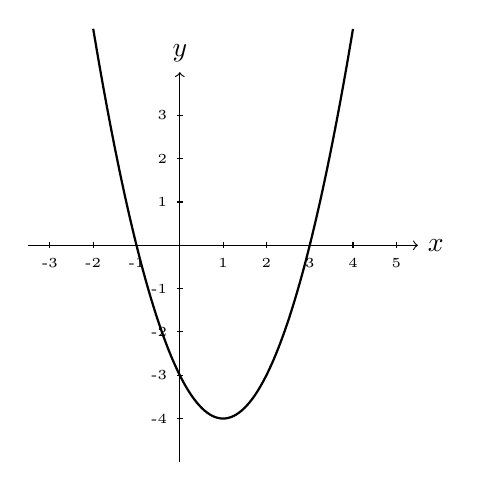
\begin{tikzpicture}[scale=0.55]
            \draw[->] (-3.5,0) -- (5.5,0) node[right] {$x$};
            \draw[->] (0,-5) -- (0,4) node[above] {$y$};
            \foreach \x in {-3,-2,-1,1,2,3,4,5} \draw (\x,0.07)--(\x,-0.07) node[below]{\tiny\x};
            \foreach \y in {-4,-3,-2,-1,1,2,3} \draw (0.07,\y)--(-0.07,\y) node[left]{\tiny\y};
            \draw[thick, domain=-2:4, smooth, samples=50] plot (\x, {(\x-1)^2 - 4});
        \end{tikzpicture}
    \end{minipage}
    \hfill
    \begin{minipage}[t]{0.40\linewidth}
        Vertex: \blank{2.5cm}\\[8pt]
        Axis of symmetry: $x =$ \blank{1.5cm}\\[8pt]
        $y$-intercept: \blank{2.5cm}\\[8pt]
        Zeros: $x =$ \blank{1cm} and $x =$ \blank{1cm}\\[8pt]
        Opens: \quad up \quad / \quad down
    \end{minipage}

    \vspace{0.2in}

    \item A scatterplot shows data points that rise from left to right. Is the trend linear or quadratic? Explain in one sentence.

    \vspace{0.5in}

\end{enumerate}
\end{tcolorbox}

\vspace{0.15in}

% ─────────────────────────────────────────────
%  TIER A — Approaching Proficiency
% ─────────────────────────────────────────────
\begin{tcolorbox}[colback=white,colframe=black!40,boxrule=0.7pt,arc=2mm,
    title={\bfseries Tier A — Approaching Proficiency},fonttitle=\small,breakable]

\begin{enumerate}

    \item Write the equation of the line through $(-2, 1)$ and $(4, 13)$ in slope-intercept form.

    \vspace{0.9in}

    \item For $f(x) = -x^2 + 6x - 5$:
    \begin{enumerate}[label=(\alph*)]
        \item Find the axis of symmetry and vertex.
        \vspace{0.6in}
        \item Find the zeros by factoring.
        \vspace{0.6in}
        \item State the domain and range.
        \vspace{0.4in}
    \end{enumerate}

    \item For $g(x) = 4 \cdot 2^x$, find $g(0)$ and $g(3)$. Then describe the domain and range.

    \vspace{0.7in}

    \item A linear regression model for a data set is $y = 3.5x + 12$.
    Interpret the slope and $y$-intercept in the context: ``$x$ = years since 2010; $y$ = thousands of subscribers.''

    \vspace{0.7in}

\end{enumerate}
\end{tcolorbox}

% ─────────────────────────────────────────────
%  TIER E — Extension
% ─────────────────────────────────────────────
\begin{tcolorbox}[colback=white,colframe=black!40,boxrule=0.7pt,arc=2mm,
    title={\bfseries Tier E — Extension},fonttitle=\small,breakable]

\begin{enumerate}

    \item Write the equation of the line through $(3, -1)$ that is perpendicular to $y = \dfrac{3}{4}x + 2$.

    \vspace{0.9in}

    \item The table below gives data for hours of exercise per week ($x$) and resting heart rate ($y$, in bpm).

    \vspace{0.1in}
    \begin{center}
    \renewcommand{\arraystretch}{1.4}
    \begin{tabular}{|c|c|c|c|c|c|c|}
    \hline
    $x$ & 1 & 2 & 3 & 4 & 5 & 6 \\
    \hline
    $y$ & 82 & 78 & 74 & 71 & 67 & 64 \\
    \hline
    \end{tabular}
    \end{center}
    \vspace{0.1in}
    \begin{enumerate}[label=(\alph*)]
        \item Enter the data in Desmos and run a linear regression. Write the equation. \blank{4cm}
        \vspace{0.3in}
        \item Interpret the slope in context.
        \vspace{0.5in}
        \item Predict the resting heart rate for someone who exercises 8 hours per week. Is this prediction reasonable?
        \vspace{0.5in}
    \end{enumerate}

    \item Compare $f(x) = 2x + 10$, $g(x) = x^2 + 2$, and $h(x) = 1.5^x$.
    For which values of $x$ is $h(x) > f(x)$? Use Desmos to find the approximate intersection, then explain.

    \vspace{0.8in}

\end{enumerate}
\end{tcolorbox}

\end{document}
